%Frame 1 Kort introduktion

\begin{frame}
  \frametitle{VGA\_driver}
  \framesubtitle{Overview}
  \begin{itemize}
  \item<1-> Based on Laboration 2.
  \item<2-> Two new submodules.
    \begin{itemize}
    \item<3-> bar\_tender.
    \item<4-> bar\_mixer.
    \end{itemize}
  \item<5-> Nånting bra testest.
  \end{itemize}
\end{frame}

%Frame 2 Överiktsbild

\begin{frame}
  \frametitle{VGA\_driver}
  \framesubtitle{System overview}
  \begin{figure}[H]
    \centering 
    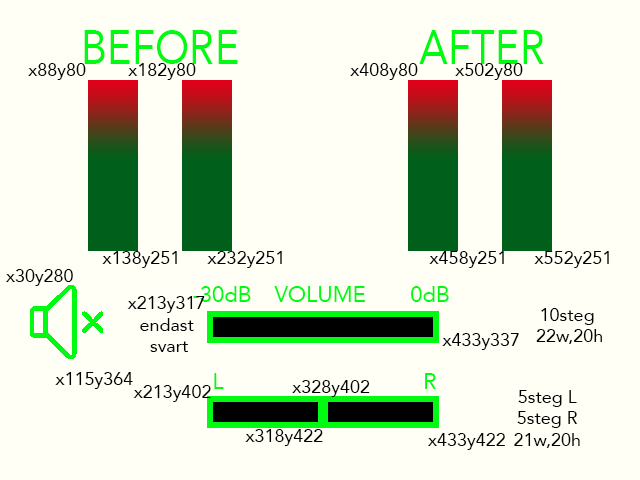
\includegraphics[scale=0.80]{picture_xy.png} 
    %\caption{Entity-Relationship diagram} 
    \label{fig:picture_xy.png}
  \end{figure}
\end{frame}

\begin{frame}
  %\begin{itemize}
  %\item<1-> test
  %\item<2-> test2
  %\end{itemize}
  
  \frametitle{VGA\_driver}
  \framesubtitle{System overview}
  \begin{figure}[l]
    \centering 
    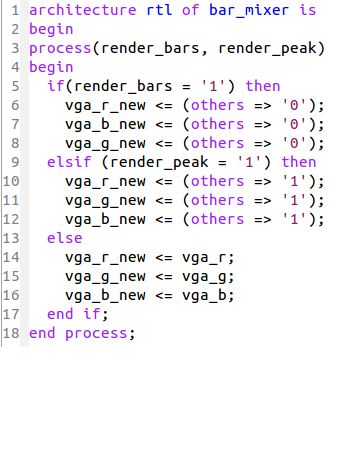
\includegraphics[scale=0.40]{bar_mixer.png} 
    %\caption{Entity-Relationship diagram} 
    \label{fig:bar_mixer.png}
  \end{figure}
\end{frame}
